%\RequirePackage{currfile}
\documentclass[12pt]{beamer}
\usepackage[utf8]{inputenc}
\usepackage[spanish]{babel}
\usepackage{standalone}
\usepackage{color}
\usepackage{siunitx}
\usepackage{hyperref}
\usepackage[outdir=./]{epstopdf}
%\hypersetup{colorlinks,linkcolor=,urlcolor=blue}
%\hypersetup{colorlinks,urlcolor=blue}
\usepackage{anyfontsize}
\usepackage{lmodern}
\usepackage{xcolor,soul}
\usepackage{etoolbox}
\usepackage{amsmath}
\usepackage{amsthm}
\usepackage{mathtools}
\usepackage{tcolorbox}
\usepackage{physics}
\usepackage{multicol}
\usepackage{bookmark}
\usepackage{longtable}
\usepackage{listings}
\usepackage{cancel}
\usepackage{wrapfig}
\usepackage{empheq}
\usepackage{graphicx}
\usepackage{tikz}
\usetikzlibrary{calc, patterns, matrix, backgrounds, decorations,shapes, arrows.meta}
\usepackage[autostyle,spanish=mexican]{csquotes}
\usepackage[os=win]{menukeys}
\usepackage{pifont}
\usepackage{pbox}
\usepackage{bm}
\usepackage{caption}
\captionsetup{font=scriptsize,labelfont=scriptsize}
%\usepackage[sfdefault]{roboto}  %% Option 'sfdefault' only if the base font of the document is to be sans serif

%Sección de definición de colores
\definecolor{ao}{rgb}{0.0, 0.5, 0.0}
\definecolor{bisque}{rgb}{1.0, 0.89, 0.77}
\definecolor{amber}{rgb}{1.0, 0.75, 0.0}
\definecolor{armygreen}{rgb}{0.29, 0.33, 0.13}
\definecolor{alizarin}{rgb}{0.82, 0.1, 0.26}
\definecolor{cadetblue}{rgb}{0.37, 0.62, 0.63}
\definecolor{deepblue}{rgb}{0,0,0.5}
\definecolor{brown}{rgb}{0.59, 0.29, 0.0}
\definecolor{OliveGreen}{rgb}{0,0.25,0}
\definecolor{mycolor}{rgb}{0.122, 0.435, 0.698}

\newcommand*{\boxcolor}{orange}
\makeatletter
\newcommand{\boxedcolor}[1]{\textcolor{\boxcolor}{%
\tikz[baseline={([yshift=-1ex]current bounding box.center)}] \node [rectangle, minimum width=1ex, thick, rounded corners,draw] {\normalcolor\m@th$\displaystyle#1$};}}
 \makeatother

 \newcommand*\widefbox[1]{\fbox{\hspace{2em}#1\hspace{2em}}}

\newtcbox{\mybox}{on line,
  colframe=mycolor,colback=mycolor!10!white,
  boxrule=0.5pt,arc=4pt,boxsep=0pt,left=6pt,right=6pt,top=6pt,bottom=6pt}

\usefonttheme[onlymath]{serif}
%Sección de definición de nuevos comandos

\newcommand*{\TitleParbox}[1]{\parbox[c]{1.75cm}{\raggedright #1}}%
\newcommand{\python}{\texttt{python}}
\newcommand{\textoazul}[1]{\textcolor{blue}{#1}}
\newcommand{\azulfuerte}[1]{\textcolor{blue}{\textbf{#1}}}
\newcommand{\funcionazul}[1]{\textcolor{blue}{\textbf{\texttt{#1}}}}
\newcommand{\ptilde}[1]{\ensuremath{{#1}^{\prime}}}
\newcommand{\stilde}[1]{\ensuremath{{#1}^{\prime \prime}}}
\newcommand{\ttilde}[1]{\ensuremath{{#1}^{\prime \prime \prime}}}
\newcommand{\ntilde}[2]{\ensuremath{{#1}^{(#2)}}}
\renewcommand{\arraystretch}{1.5}

\newcounter{saveenumi}
\newcommand{\seti}{\setcounter{saveenumi}{\value{enumi}}}
\newcommand{\conti}{\setcounter{enumi}{\value{saveenumi}}}
\renewcommand{\rmdefault}{cmr}% cmr = Computer Modern Roman

\linespread{1.5}

\usefonttheme{professionalfonts}
%\usefonttheme{serif}
\DeclareGraphicsExtensions{.pdf,.png,.jpg}

%Sección para el tema de beamer, con el theme, usercolortheme y sección de footers
\mode<presentation>
{
  \usetheme{Berlin}
  
  %\useoutertheme{infolines}
  \useoutertheme{default}
  \usecolortheme{beaver}
  \setbeamercovered{invisible}
  % or whatever (possibly just delete it)
  \setbeamertemplate{section in toc}[sections numbered]
  \setbeamertemplate{subsection in toc}[subsections numbered]
  \setbeamertemplate{subsection in toc}{\leavevmode\leftskip=3.2em\rlap{\hskip-2em\inserttocsectionnumber.\inserttocsubsectionnumber}\inserttocsubsection\par}
  \setbeamercolor{section in toc}{fg=blue}
  \setbeamercolor{subsection in toc}{fg=blue}
  \setbeamercolor{frametitle}{fg=blue}
  \setbeamertemplate{caption}[numbered]

  \setbeamertemplate{footline}
  \beamertemplatenavigationsymbolsempty
  \setbeamertemplate{headline}{}
}

\makeatletter
\setbeamercolor{section in foot}{bg=gray!30, fg=black!90!orange}
\setbeamercolor{subsection in foot}{bg=blue!30!yellow, fg=red}
\setbeamertemplate{footline}
{
  \leavevmode%
  \hbox{%
  \begin{beamercolorbox}[wd=.333333\paperwidth,ht=2.25ex,dp=1ex,center]{section in foot}%
    \usebeamerfont{section in foot} \insertsection
  \end{beamercolorbox}}%
  \begin{beamercolorbox}[wd=.333333\paperwidth,ht=2.25ex,dp=1ex,center]{subsection in foot}%
    \usebeamerfont{subsection in foot}  \insertsubsection
  \end{beamercolorbox}%
  \begin{beamercolorbox}[wd=.333333\paperwidth,ht=2.25ex,dp=1ex,right]{date in head/foot}%
    \usebeamerfont{date in head/foot} \insertshortdate{} \hspace*{2em}
    \insertframenumber{} / \inserttotalframenumber \hspace*{2ex} 
  \end{beamercolorbox}}%
  \vskip0pt%
\makeatother  

\makeatletter
\patchcmd{\beamer@sectionintoc}
  {\vfill}
  {\vskip\itemsep}
  {}
  {}
\makeatother


\title{\large{Aplicaciones de la Transformada de Fourier}}
\subtitle{Tema 6 - Transformadas Integrales}
\author{M. en C. Gustavo Contreras Mayén}
\date{}
\institute{Facultad de Ciencias - UNAM}
\titlegraphic{\includegraphics[width=1.75cm]{../Imagenes/escudo-facultad-ciencias}\hspace*{4.75cm}~%
   \includegraphics[width=1.75cm]{../Imagenes/escudo-unam}
}
\setbeamertemplate{navigation symbols}{}
\usepackage{scalerel}
\def\scaleint#1{\vcenter{\hbox{\scaleto[3ex]{\displaystyle\int}{#1}}}}
\def\bs{\mkern-12mu}

\begin{document}
\maketitle
\fontsize{14}{14}\selectfont
\spanishdecimal{.}

\section*{Contenido}
\frame[allowframebreaks]{\tableofcontents[currentsection, hideallsubsections]}

\section{Áreas de aplicación}
\frame{\tableofcontents[currentsection, hideothersubsections]}
\subsection{Uso de la Transformada de Fourier}

\begin{frame}
\frametitle{Introducción}
Las aplicaciones de la Transformada de Fourier (TF) son muy extensas, ya que abarcan diversas ramas de la física matemática.
\end{frame}
\begin{frame}
\frametitle{Introducción}
Desde la teoría de números y geometría hasta óptica y mecánica cuántica, así como otras áreas de la ciencia tales como: la medicina, comunicaciones, ingeniería biomédica, ingeniería mecánica y de control, campos electromagnéticos, procesamiento de señales de audio y procesamiento de imágenes.
\end{frame}
\begin{frame}
\frametitle{Usos de la TF}
La TF también se utiliza para:
\setbeamercolor{item projected}{bg=blue!70!black,fg=yellow}
\setbeamertemplate{enumerate items}[circle]
\begin{enumerate}[<+->]
\item Analizar contenido de frecuencia de las señales.
\item Determinar como cambia la amplitud y las fases de las señales sinusoidales cuando éstas pasan a través de un sistema lineal e invariante en el tiempo.
\seti
\end{enumerate}
\end{frame}
\begin{frame}
\frametitle{Usos de la TF}
\setbeamercolor{item projected}{bg=blue!70!black,fg=yellow}
\setbeamertemplate{enumerate items}[circle]
\begin{enumerate}[<+->]
\conti
\item Generar formas de onda de corriente o tensión eléctrica por medio de la superposición de señales senoidales generadas por osciladores electrónicos de amplitud variable cuyas frecuencias ya están determinadas.
\item Analizar el comportamiento armónico de una señal.
\end{enumerate}
\end{frame}

\subsection{Ejemplos concretos}

\begin{frame}
\frametitle{Electromagnetismo y de microondas}
La Transformada de Fourier está relacionada con:
\begin{itemize}[<+->]
\item El cálculo del campo cercano transitorio irradiado por dispositivos electrónicos.
\item El análisis de fenómenos ópticos en microondas.
\item El cálculo del campo electromagnético de rayos, la formación de haz y la radiación de microondas solares.
\end{itemize}
\end{frame}
\begin{frame}
\frametitle{Medicina}
El análisis de la TF está relacionado con:
\begin{itemize}[<+->]
\item El análisis espectral del comportamiento global de los cromosomas.
\item El análisis espectral de la variabilidad de la frecuencia cardíaca.
\item El procesamiento de imágenes generadas por econogramas, resonancias magnéticas y tomografía axial.
\end{itemize}
\end{frame}
\begin{frame}
\frametitle{Comunicaciones}
Se usa para:
\begin{itemize}[<+->]
\item Analizar la frecuencia de señales.
\item Diseñar los sistemas de transmisión de señales para transmitir información.
\item Diseñar supresores y canceladores de ecos en líneas telefónicas.
\end{itemize}
\end{frame}
\begin{frame}
\frametitle{Ingeniería mecánica}
\begin{itemize}[<+->]
\item  Se utiliza para balancear rotores y eliminar la vibración que se genera cuando no están balanceados.
\item Estudiar los problemas relacionados con vibraciones mecánicas en los motores, generadores y equipos rotatorios en general.
\end{itemize}
\end{frame}
\begin{frame}
\frametitle{Procesamiento de señales de audio}
\begin{itemize}[<+->]
\item Se usa para compactar las señales de audio (formatos MP3 y MP4).
\item Producir efectos de sonido, diseñar sintetizadores de audio y ecualizadores.
\end{itemize}
\end{frame}
\begin{frame}
\frametitle{Procesamiento de imágenes}
\begin{itemize}[<+->]
\item La TF se utiliza para filtrar imágenes, extraer características de interés.
\item Realizar transformaciones de imágenes y compactar imágenes.
\end{itemize}
\end{frame}
\begin{frame}
\frametitle{Usando filtros}
Algo de lo que podemos hacer con la TF de una imagen es eliminar algunos componentes.
\\
\bigskip
\pause
Si eliminamos las frecuencias bajas, menores de cierto valor $\omega_{f}$, se le llama \textbf{filtro de paso alto}. \pause Una gran cantidad de ruido de fondo se produce a bajas frecuencias, por lo que un filtro de paso alto puede limpiar una señal.
\end{frame}
\begin{frame}
\frametitle{Filtro pasa bajos}
 Si descartamos las frecuencias altas, se llama \emph{filtro de paso bajo}.
 \\
 \bigskip
 \pause
 Se puede usar un filtro de paso bajo para suavizar los datos (como una foto digital), ya que arroja ruido de alta frecuencia.
 \pause

 Un filtro que corta las frecuencias altas y bajas se llama \emph{filtro de paso de banda}.
\end{frame}
\begin{frame}
\frametitle{Ejemplo de filtro pasa altos}
\centering
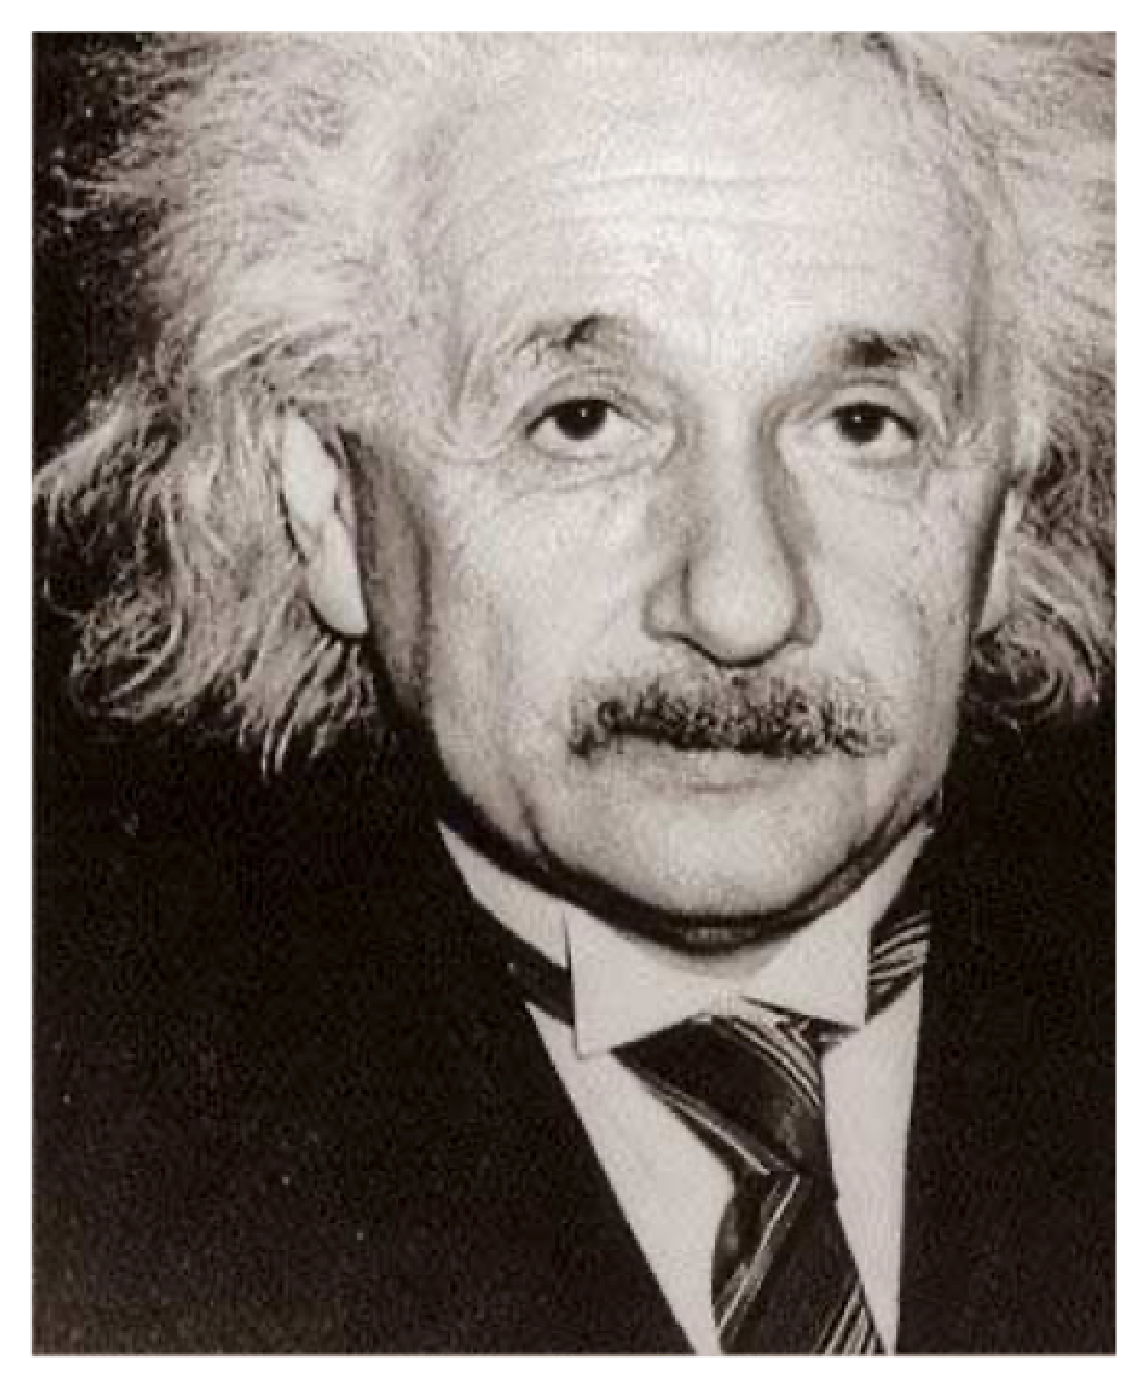
\includegraphics[scale=0.27]{Imagenes/Einstein_01.eps}
\pause
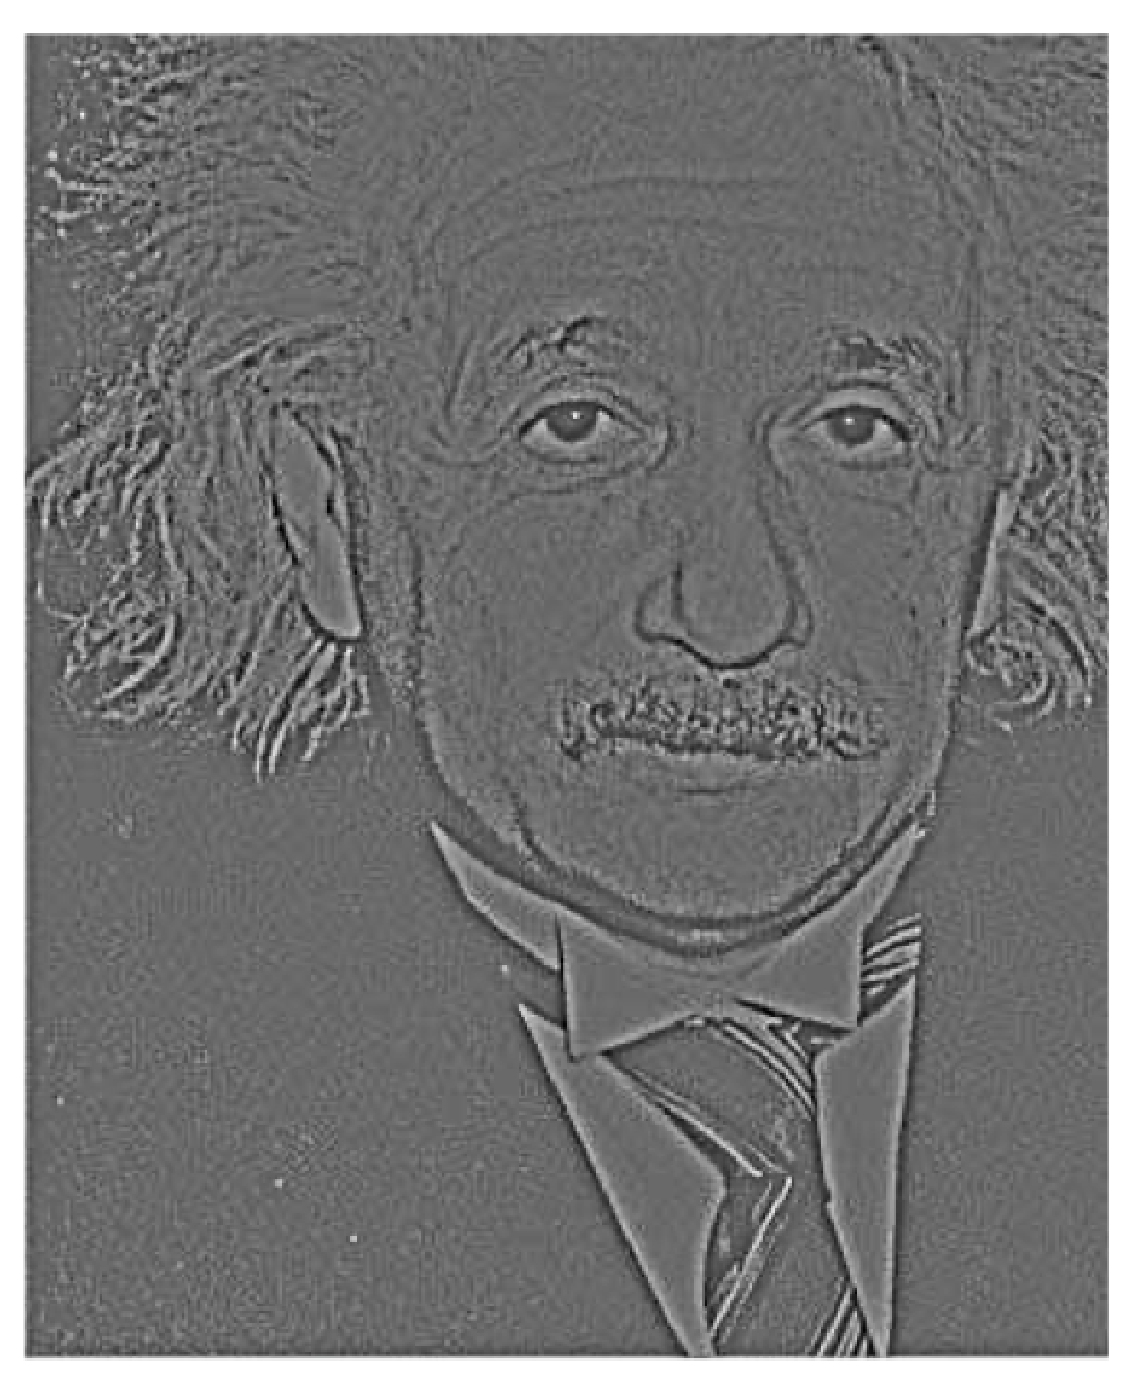
\includegraphics[scale=0.27]{Imagenes/Einstein_02.eps}
\end{frame}
\begin{frame}
\frametitle{Ejemplo de filtro pasa bajos}
\centering
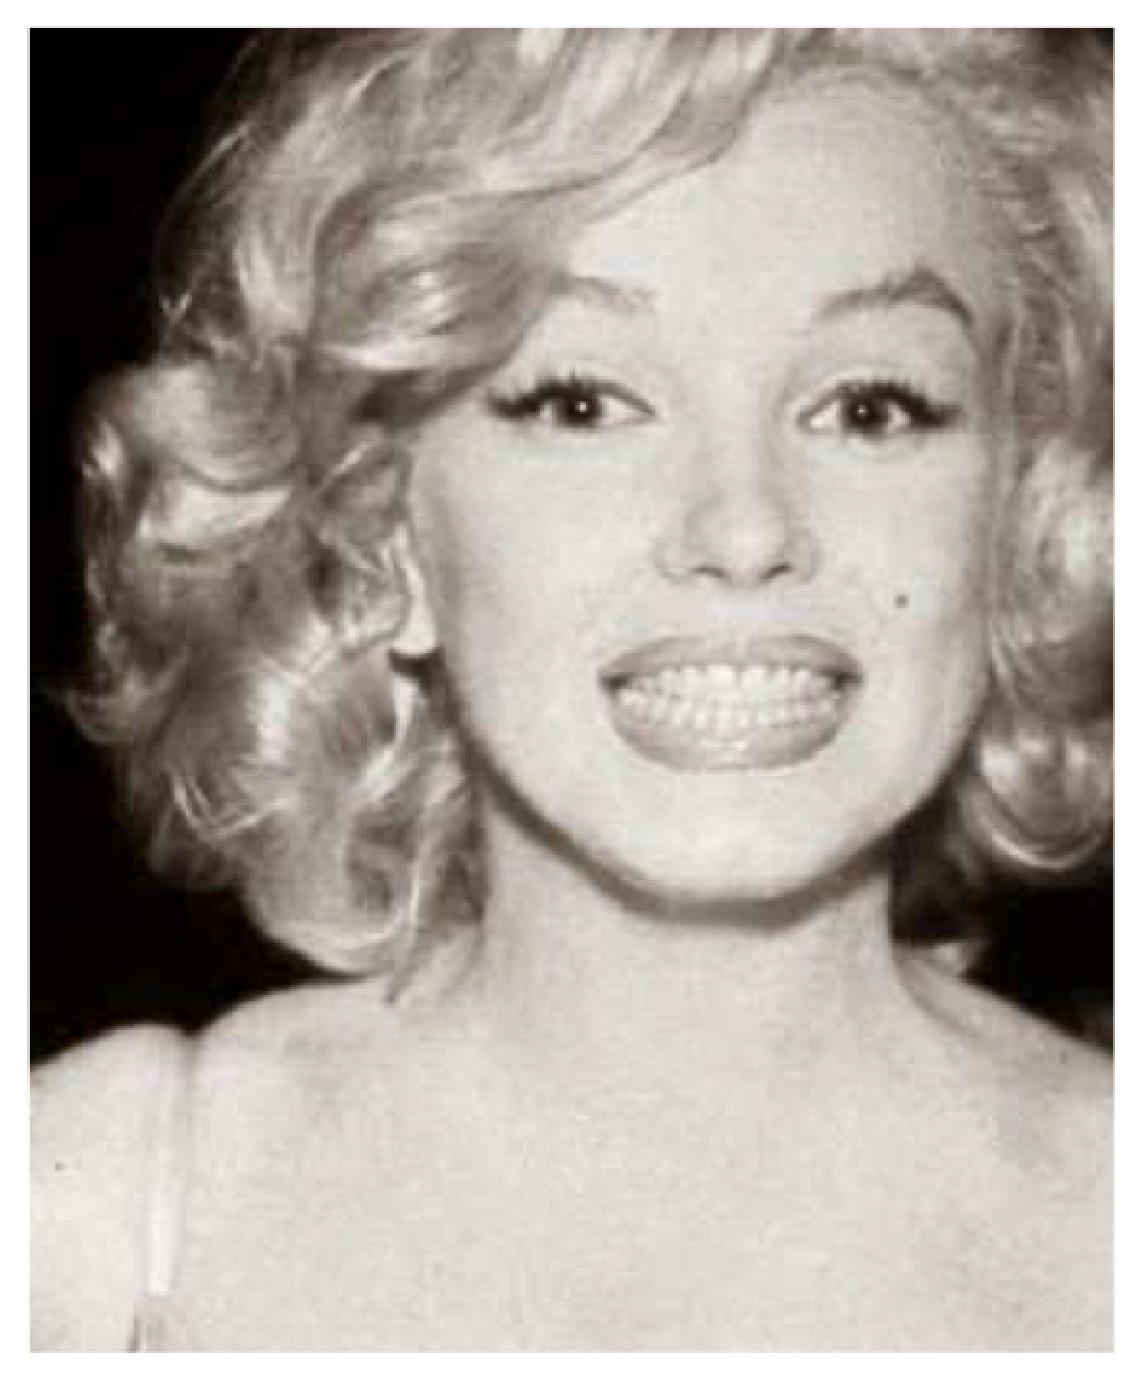
\includegraphics[scale=0.27]{Imagenes/Marylin_01.eps}
\pause
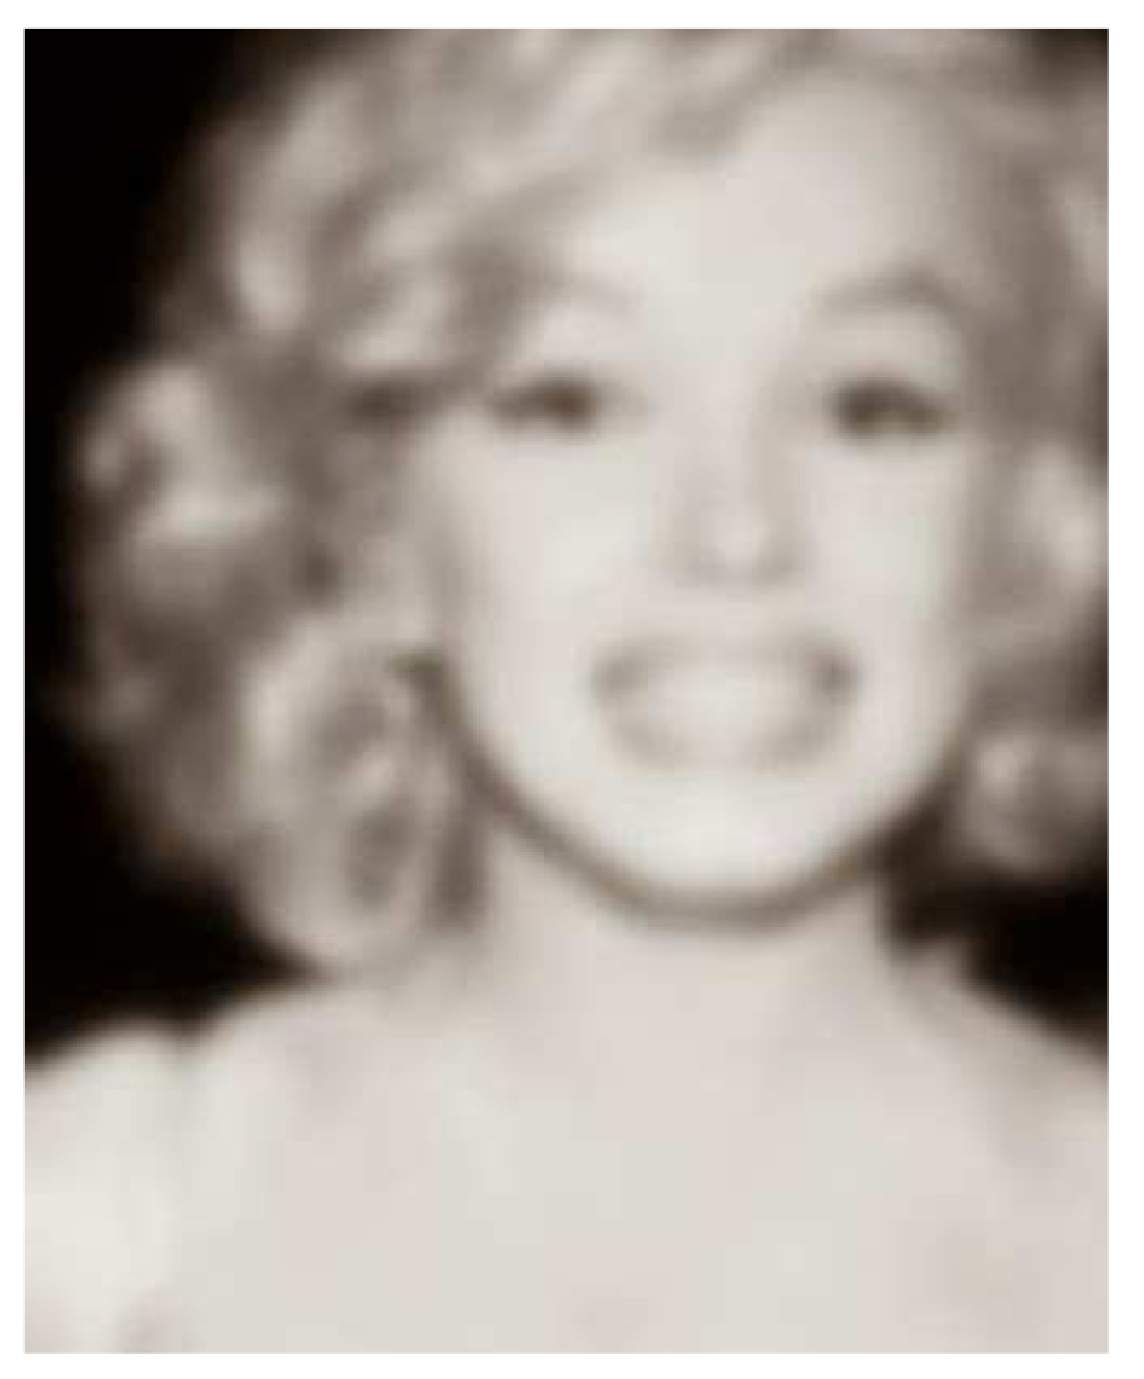
\includegraphics[scale=0.27]{Imagenes/Marylin_02.eps}
\end{frame}
\begin{frame}
\frametitle{Combinando los filtros}
\begin{figure}
    \centering
    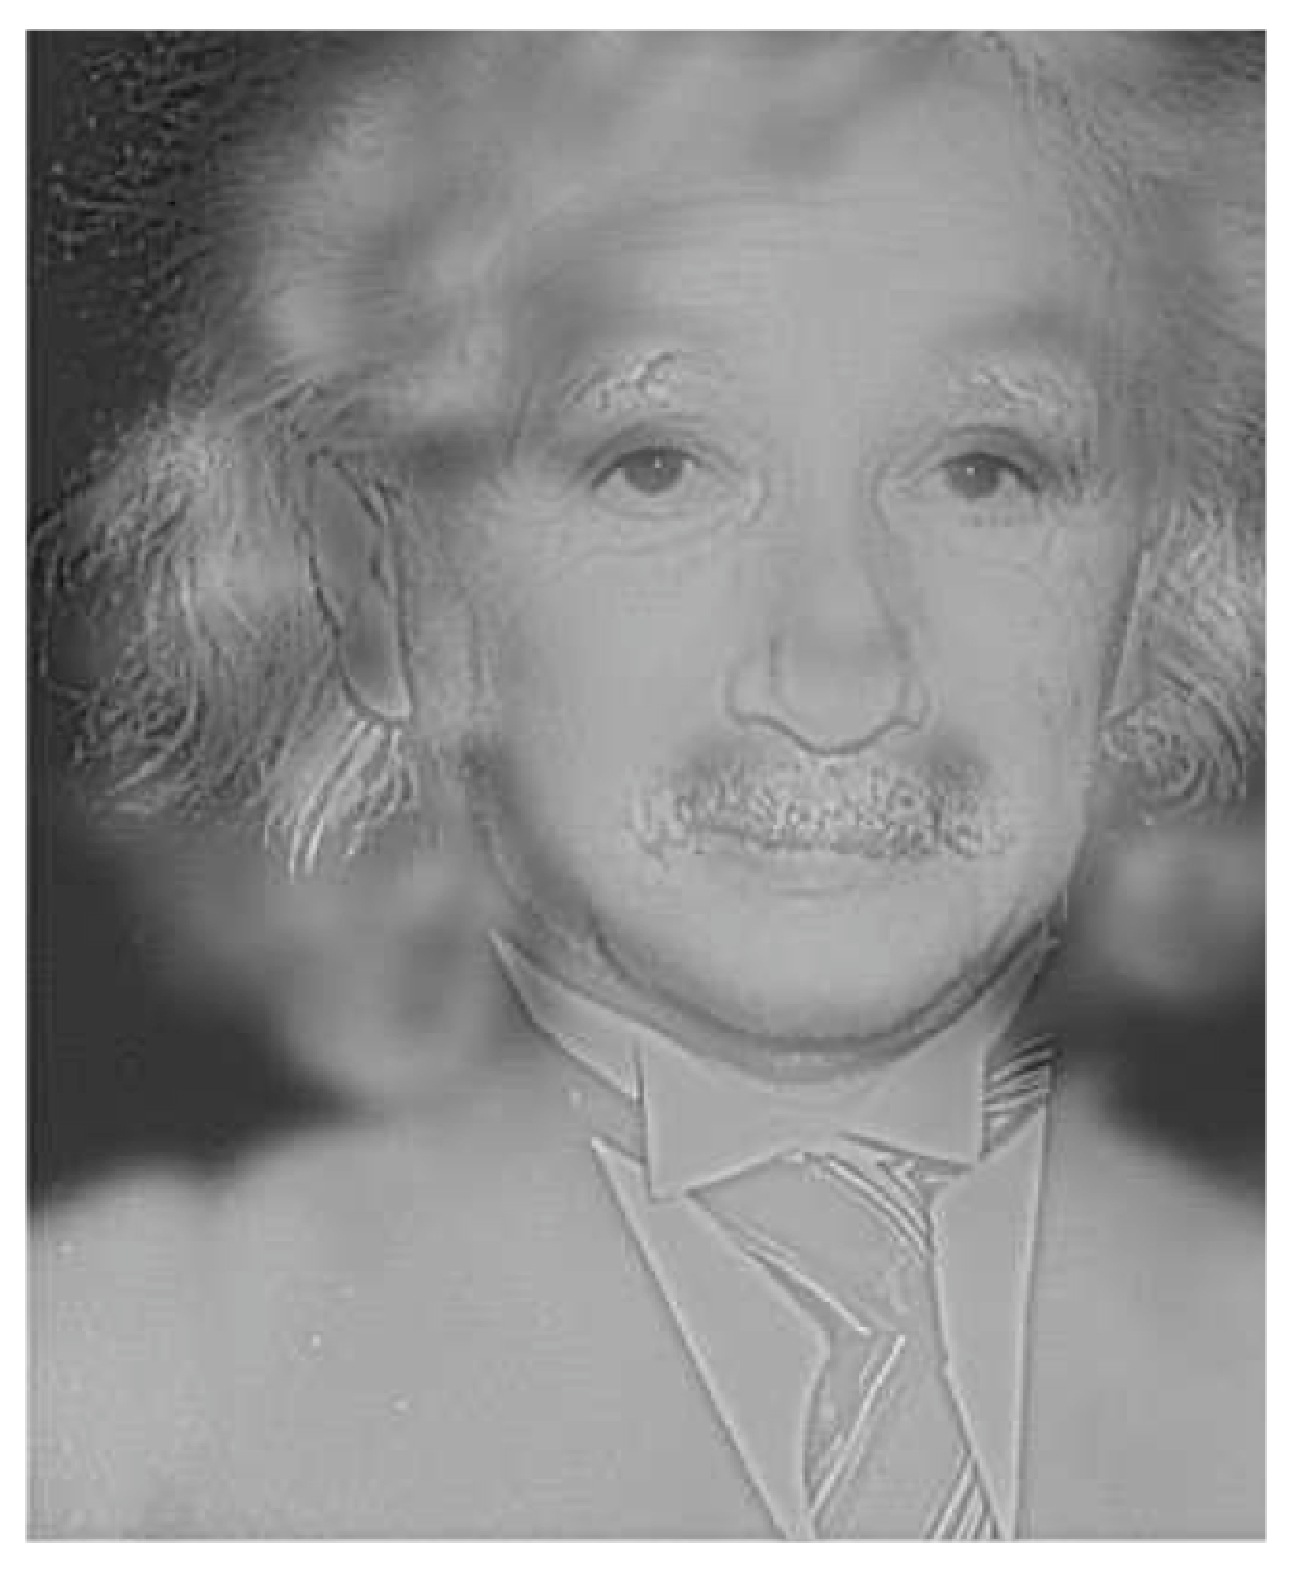
\includegraphics[scale=0.22]{Imagenes/Einstein_Marylin_AB_01.eps}
    \caption{Filtro pasa alto Einstein + pasa bajo Marylin}
\end{figure}
\end{frame}
\begin{frame}
\frametitle{Combinando los filtros}
\begin{figure}
    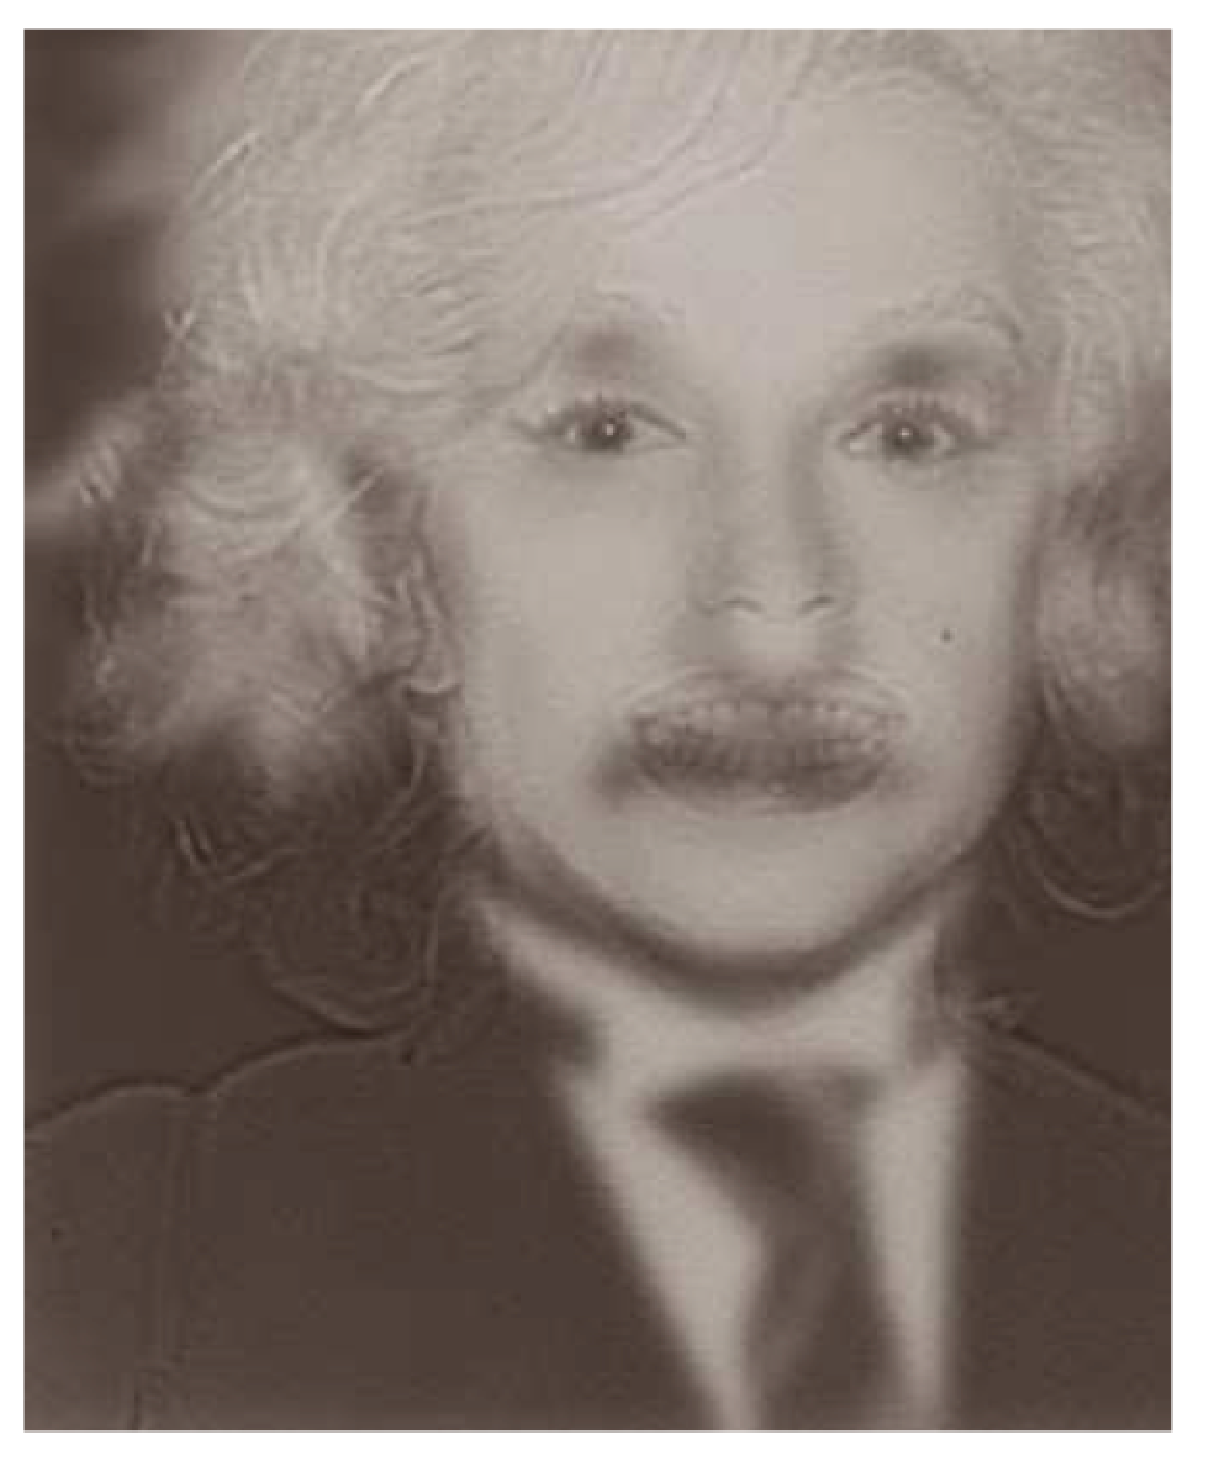
\includegraphics[scale=0.25]{Imagenes/Einstein_Marylin_BA_01.eps}
    \caption{Filtro pasa bajo Einstein + pasa alto Marylin}
\end{figure}
\end{frame}

\section{Transformada de Fourier}
\frame{\tableofcontents[currentsection, hideothersubsections]}
\subsection{Definición}

\begin{frame}
\frametitle{La transformada de Fourier}
Se define la transformada de Fourier como:
\begin{align}
F \big[ f(x); x \to \xi \big] = \dfrac{1}{\sqrt{2 \, \pi}} \scaleint{5ex}_{\bs -\infty}^{+\infty} f(x) \, \exp(i \, \xi \, x) \dd{x}
\label{eq:ecuacion_01_12}
\end{align}
\end{frame}
\begin{frame}
\frametitle{La transformada inversa de Fourier}
Se define la transformada inversa de Fourier como:
\begin{align}
f(x) = F^{-1} \big[ F(\xi) \big] = \dfrac{1}{\sqrt{2 \, \pi}} \int_{-\infty}^{+\infty} F(\xi) \, \exp(-i \, \xi \, x) \dd{\xi}
\label{eq:ecuacion_01_13}
\end{align}
en un punto continuo de $f(x)$.
\end{frame}

\subsection{Ejercicios con la TF}

\begin{frame}
\frametitle{Calculando la transformada de Fourier}
Evalúa la transformada de Fourier de:
\begin{align*}
f(x) = \begin{cases}
x, & \abs{x} < a \\
0, & \abs{x} > a
\end{cases}
\end{align*}
\pause
Ocupamos la definición de la transformada de Fourier, ec. (\ref{eq:ecuacion_01_12}).
\end{frame}
\begin{frame}
\frametitle{Definición de la TF}
Por la definición de la TF:
\begin{align*}
F \big[ f(x); x \to \xi \big] = \dfrac{1}{\sqrt{2 \, \pi}} \scaleint{5ex}_{\bs -a}^{a} x \, \exp(i \, \xi \, x) \dd{x}
\end{align*}
\pause
Resolvemos la integral por partes.
\end{frame}
\begin{frame}
\frametitle{Integración por partes}
Se tiene que:
\pause
\begin{eqnarray*}
&=& \dfrac{1}{\sqrt{2 \, \pi}} \left\{ \bigg[ x \, \dfrac{\exp(i \, \xi \, x)}{i \, \xi} \bigg] \bigg\vert_{-a}^{a} - \dfrac{1}{i \, \xi} \scaleint{5ex}_{\bs -a}^{a} \exp(i \xi \, x) \dd{x} \right\} \\[1em] \pause
&=& \dfrac{1}{\sqrt{2 \, \pi}} \bigg[ \dfrac{a \, e^{i \xi a} + a \, e^{-i \xi a}}{i \, \xi} + \dfrac{1}{\xi^{2}} \left( e^{i a \xi} - e^{-i a \xi} \right) \bigg] =
\end{eqnarray*}
\end{frame}
\begin{frame}
\frametitle{Reduciendo términos}
Ocupando identidades conocidas, se tiene que:
\pause
\begin{eqnarray*}
&=& \dfrac{1}{\sqrt{2 \, \pi}} \bigg[ \dfrac{2 \, a \, \cos a \xi}{i \, \xi} + \dfrac{2 \, i \, \sin a \xi}{\xi^{2}} \bigg] = \\[1em] \pause
&=& \sqrt{\dfrac{2}{\pi}} \, i \, \bigg[ \dfrac{\sin a \xi - a \, \xi \, \cos a \, \xi}{\xi^{2}} \bigg]
\end{eqnarray*}
\end{frame}

\begin{frame}
\frametitle{Otro Ejercicio}
Calcula la transformada de Fourier de:
\begin{align*}
f(x) = \exp(-a \, \abs{x}), \hspace{1cm} a > 0
\end{align*}
\pause
Ocupamos nuevamente la definición de la TF.
\end{frame}
\begin{frame}
\frametitle{Ocupando la definición de la TF}
Con la definición de TF se tiene que:
\pause
\begin{align*}
F \big[ f(x); x \to \xi \big] {=} \dfrac{1}{\sqrt{2 \pi}} \scaleint{5ex}_{\bs -\infty}^{+\infty} \exp(-a \abs{x}) \, \exp(i \xi x) \dd{x}
\end{align*}
Para resolver la integral, primero \enquote{separamos} en el dominio el integrando:
\end{frame}
\begin{frame}
\frametitle{Separando la integral}
\begin{eqnarray*}
&=& \dfrac{1}{\sqrt{2 \pi}} \bigg[ \scaleint{5ex}_{\bs -\infty}^{0} e^{ a  x} \, e^{i \xi x} \dd{x} + \scaleint{5ex}_{\bs 0}^{\infty} e^{ -a  x} \, e^{i \xi x} \dd{x} \bigg] =
\end{eqnarray*}
\pause
Cada integral se resuelve directamente y se evalúa en los límites de integración.
\end{frame}
\begin{frame}
\frametitle{Resultado}
Se obtiene entonces:
\pause
\begin{eqnarray*}
&=& \dfrac{1}{\sqrt{2 \pi}} \bigg[ \dfrac{1}{a + i \, \xi} + \dfrac{1}{a - i \xi} \bigg] = \\[0.5em] \pause
&=& \sqrt{\dfrac{2}{\pi}} \dfrac{a}{a^{2} + \xi^{2}}
\end{eqnarray*}
\end{frame}

\section{Ecuación de calor}
\frame{\tableofcontents[currentsection, hideothersubsections]}
\subsection{Temperatura en una placa semiinfinita}

\begin{frame}
\frametitle{Enunciado}
La temperatura constante de una placa semiinfinita está dada por la siguiente ecuación diferencial, condiciones iniciales y de frontera:
\begin{align*}
&\pdv[2]{u}{x} + \pdv[2]{u}{y} = 0 \hspace{1cm} 0 < x < \pi, \hspace{0.3cm} y > 0 \\[0.5cm]
&u(0, y) = 0 \hspace{1cm} u(\pi, y) = e^{-y} \hspace{0.3cm} y > 0 \\[0.5cm]
&\pdv{u}{y} \eval_{y=0} = 0 \hspace{1cm} 0 < x < \pi
\end{align*}
\end{frame}
\begin{frame}
\frametitle{Problema a resolver}
\textbf{Encuentra el valor de temperatura de $u(x,y)$}.
\end{frame}
\begin{frame}
\frametitle{Solución}
El dominio de la variable y la condición prescrita en $y = 0$, indican que se puede aplicar la transformada coseno de Fourier al problema, así:
\begin{align*}
F_{c} \big[u(x,y)\big] = \scaleint{5ex}_{\bs 0}^{\infty} u(x, y) \, \cos \alpha \, y \dd{y} = U(x, \alpha)
\end{align*}
\end{frame}
\begin{frame}
\frametitle{Usando un resultado}
Como la transformada coseno de Fourier de la derivada de una función es:
\begin{align*}
F_{c} \big[\stilde{y}(x)] = - \alpha^{2} \, F[\alpha] - \ptilde{f} (0)
\end{align*}
se tiene que:
\begin{align*}
F_{c} \left[\pdv[2]{u}{x} \right] + F_{c} \left[\pdv[2]{u}{y} \right] = F_{c} [0]
\end{align*}
\end{frame}
\begin{frame}
\frametitle{Expresión de la TF}
Por lo tanto:
\begin{align*}
\dv[2]{U}{x} - \alpha^{2} \, &U(x, \alpha) - u_{y} (x, 0) = 0 \\[1em]
&\Rightarrow \hspace{0.3cm} \dv[2]{U}{x} - \alpha^{2} \, U = 0
\end{align*}
\end{frame}
\begin{frame}
\frametitle{Manejo conveniente}
Puesto que el dominio de $x$ es un intervalo finito, es preferible escribir la solución a la EDO como:
\begin{align}
U(x, \alpha) = c_{1} \, \cosh (\alpha \, x) + c_{2} \, \sinh (\alpha \, x)
\label{eq:ecuacion_016}
\end{align}
\end{frame}
\begin{frame}
\frametitle{Transformada coseno de Fourier}
Ahora bien:
\begin{align*}
F_{c} \big[ u(0, y)\big] &= F_{c} [0] \\[0.5em]
F_{c} \big[ u(\pi, y)\big] &= F_{c} \big[ e^{-y} \big]
\end{align*}
son equivalentes a
\begin{align*}
U(0, \alpha) &= 0 \\[0.5em]
U(\pi, \alpha) &= \dfrac{1}{1 +  \alpha^{2}}
\end{align*}
respectivamente.
\end{frame}
\begin{frame}
\frametitle{Las constantes}
Cuando se aplican estas últimas condiciones, en la solución ec. (\ref{eq:ecuacion_016}) nos devuelve:
\begin{align*}
c_{1} &= 0 \\[0.5em]
c_{2} &= \dfrac{1}{(1 + \alpha^{2}) \, \sinh \alpha \pi}
\end{align*}
\end{frame}
\begin{frame}
\frametitle{La solución en el espacio $\alpha$}
Por lo tanto
\begin{align*}
U(x, \alpha) = \dfrac{\sinh \alpha \, x}{(1 + \alpha^{2}) \, \sinh \alpha \pi}
\end{align*}
\end{frame}
\begin{frame}
\frametitle{Usando la transformada inversa}
De modo que al ocupar la transformada coseno inversa de Fourier:
\pause
\begin{align*}
F_{c}^{-1} \big[F(\alpha)\big] = \dfrac{2}{\pi} \scaleint{5ex}_{\bs 0}^{\infty} F[\alpha] \, \cos \alpha \, x \dd{x}
\end{align*}
\end{frame}
\begin{frame}
\frametitle{Resultado en el espacio inicial}
Obtenemos el siguiente resultado:
\pause
\begin{align*}
u(x, y) = \dfrac{2}{\pi} \scaleint{6ex}_{\bs 0}^{\infty} \dfrac{\sinh \alpha \, x}{(1 + \alpha^{2}) \, \sinh \alpha \pi} \, \cos \alpha \, x \dd{x}
\end{align*}
La solución obtenida se le conoce como \emph{solución fundamental}.
\end{frame}
\end{document}